\documentclass[a4paper]{article}

\usepackage[english]{babel}
\usepackage[utf8]{inputenc}
\usepackage{amsmath}
\usepackage{graphicx}
\usepackage[colorinlistoftodos]{todonotes}

\title{Assinment39}

\author{pebj, smot}

\date{\today}

\begin{document}
\maketitle

\section{Part I - OOSE}
\subsection{Architectual style}
\label{sec:style}

\textbf{Why have we chosen the client/server architecture?}\\
We have chosen the client/server architecture style because we need to have constantly running services to notify a user when an event comes up etc. This architecture fits this scenario because it is possible to have that running on a server constantly, but not on a client which can't be expected to have the program open constantly.\\
Another reason is that we can have a database and have code that a client won't be able to see or manipulate, thus allowing us to prevent a user to harm the system and its other users. \\
Additional explanations is given by the benefits below that we have deemed more interesting than the drawbacks.\\

\textbf{Benefits:}
A server will be able to handle security manners in a way, so that the client won't be able to harm the system and its other clients. For example, accesing a
database won't need the client to hold a database connectionstring that could be sniffed/hacked out of the program. Also, because of
this architure, code execution like database manipulation can be more centrallized rather than being executed from each client or different services etc. and in that sense, a server can also function as a respiratory architure.\\
Another benefit is that by having a server handling the database etc. it can be minimized what the client needs to send and receive, thereby possibly increasing performance for a client with bad network connection.\\

\textbf{Drawbacks:}
Each service in the system runs on its own and is therefore susceptible to either being attacked individually or breaking down.
If the services is dependent on some state of another service and that one break down, it could possibly corrupt the system.\\
Another drawback is with performance which will strongly rely on the client-server connection speed. If a massive amount of data was
to be transmitted regurally with a bad connection, it could harm the performance potentially.\\


\subsection{Design goals}

\begin{itemize}
\item \textit{Usability}
To integrate CALENDAR in the users daily activities, the interface and functionality have to be kept simple and intuitive. This design goal is a refinement of the nonfunctional requirement “Usability”.
\item \textit{High availability}
For better user interaction it should be possible for the clients to access our system form as many places and as often as possible.
\item \textit{High Reliability}
No potential issues may accur during dayly usage that would make it impossible to do a use case. This design goal is a refinement of the nonfunctional requirement “Reliability”.
\item \textit{Stable response time}
The system' "response time" may not increase with increasing numbers of users or events, Therefsore the CALENDAR should support a growing user base. Performance should be as close to constant  as possible. This design goal is a refinement of the nonfunctional requirement “Performance”.
\item \textit{High extensibility}
It should be possible to extend key sectors of the system. Thus a feature in addition to notifications should be addable without having
to alter the code nessesary for the notification task etc. to work. This design goal is a refinement of the nonfunctional requirement “Supportability”.
\item \textit{High portability}
To maximize the availability of CALENDAR it has to be availablee on as many of the users platforms as possible. This design goal is a refinement of the nonfunctional requirement “Implementation”.
\end{itemize}

\subsection{Decomposition}

\begin{figure}
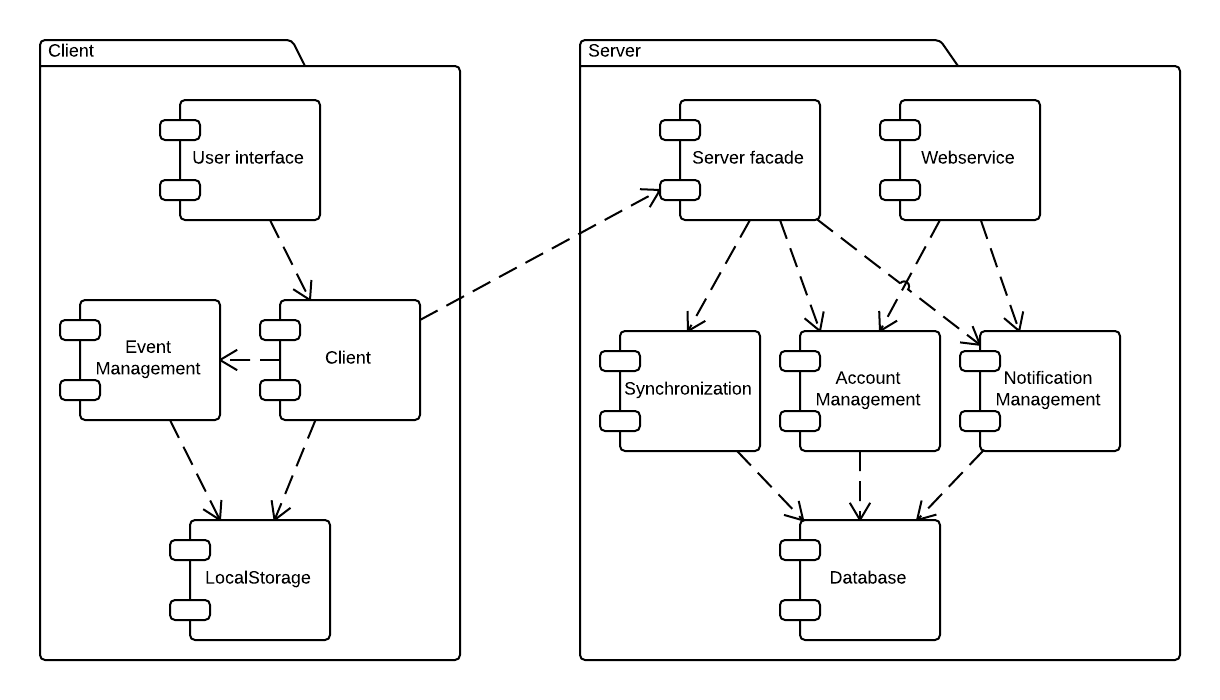
\includegraphics[scale = 0.3]{Subsystems.png}
\caption{CALENDAR subsystem decomposition (UML component diagram)}
\label{fig:decomposition}  % Figure \ref{fig:decomposition}
\end{figure}

As stated in section \ref{sec:style} the general architecture, is divided in two. The Client responsible for event management and user interactions as add new event, looking at the calendar, and the Server which stores events, accounts, notifications and notifying users. Both parts are shown in Figure \ref{fig:decomposition} with there subsystems.

The Client part design is based on a three-tier architectural style, to enables easier development or modification of different user interfaces, without changing to much of the application, to satisfy som of our design goals (e.g., Usability, portability) The application logic layer is dedicated to communication with the server and managing events. In the storage layer, the subsystem LocalStorage is responsible for storing local copies of data and changes. Together all the subsystems of the Client, starts and stores prograss of all use cases related to the user.

The Server part contains the Server facade subsystem that manages the requests from the Client and delegates requests to nested subsystems for entity storage and synchronization. Various nested subsystems are responsible for operations dealing with Synchronization, Accounts and Notifications. Which all are stored by the Database subsystem.

\end{document}